\subsection{General description}\label{subsec:general-description}

The sum of muscle activations over time during the lifting task is characterized by two peaks (Figure~\ref{fig:general_sum}, left panel).
The first peak ($454 \pm 210$\%~MVC) appears in the middle of the pulling phase (9\% of the trial) while a higher second peak ($694 \pm 343$\%~MVC) appears in the middle of the dropping phase (71\% of the trial).
The sum of muscle forces follows a similar pattern (Figure~\ref{fig:general_sum}, right panel).
A first peak ($1805 \pm 728$~N) occurs in the middle of the pulling phase and a second peak ($2858 \pm 1303$~N) in the middle of the dropping phase.

\begin{figure}[H]
    \centering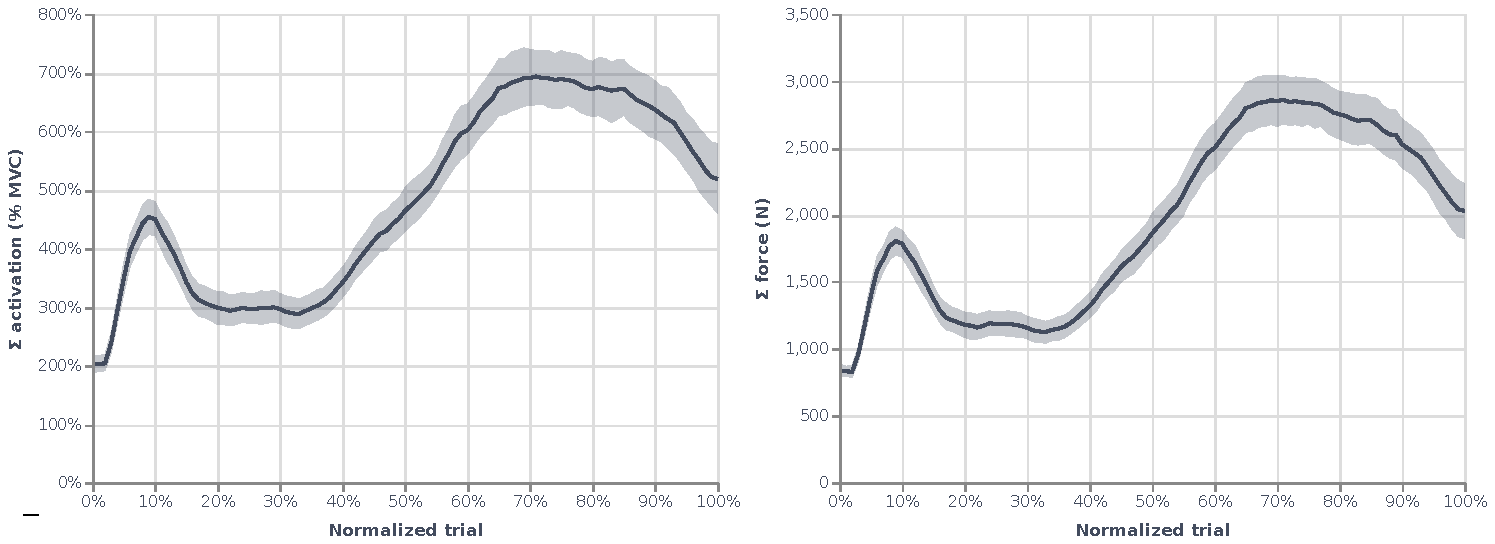
\includegraphics[width=1\linewidth]{fig/sum_general.pdf}
    \caption{Mean (lines) and 95\% confidence interval (areas) of the sum of muscle activations (left panel) and sum of muscle forces (right panel) over time.}
    \label{fig:general_sum}
\end{figure}

With regard to the density of muscle activations of all muscles (Figure~\ref{fig:general_ecdf}, left panel), half of the data is associated with low activation ($1 \pm 0$\%~MVC) while the other half has higher activation ($31 \pm 31$\%~MVC).
About 60\% of the data are below $7 \pm 5$\%~MVC, 80\% of the data are below $35 \pm 23$\%~MVC and 100\% are below $95 \pm 10$~\% MVC\@.
The density of the muscle forces (Figure~\ref{fig:general_ecdf}, right panel) is also delimited by half of the data associated with a low forces ($4 \pm 3$~N) and the other half with higher forces ($125 \pm 149$~N).
About 60\% of the data are below $23 \pm 11$~N, 80\% of the data are below $110 \pm 33$~N and 100\% below $554 \pm 216$~N\@.

\begin{figure}[H]
    \centering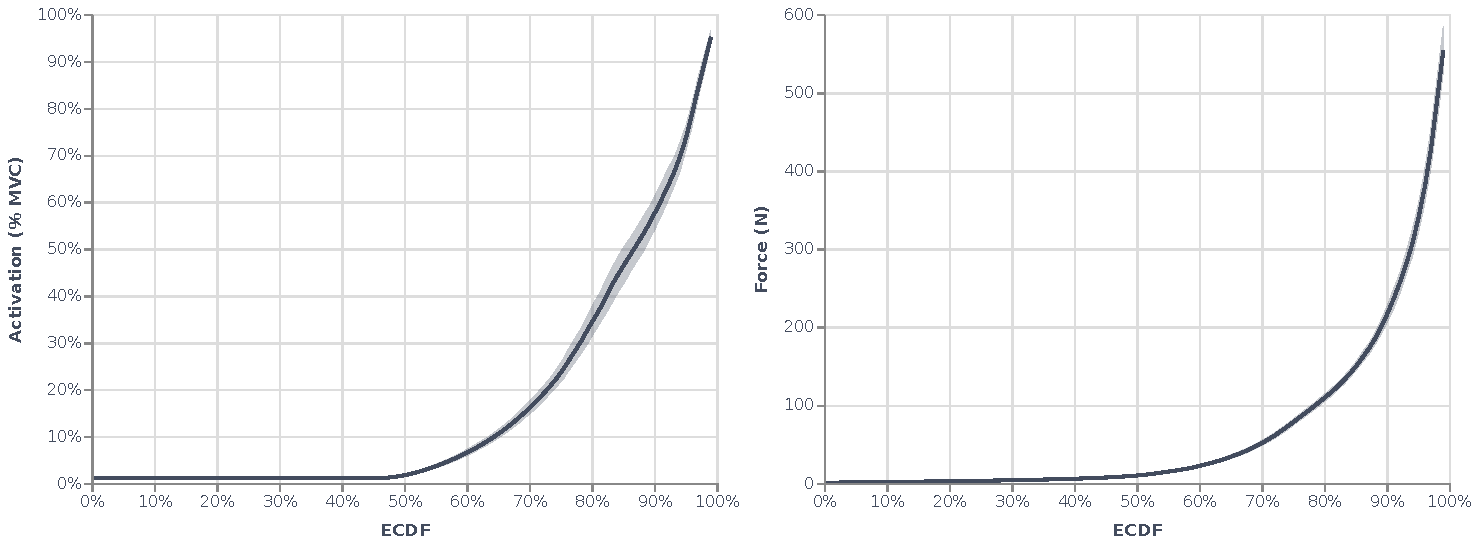
\includegraphics[width=1\linewidth]{fig/ecdf_general.pdf}
    \caption{Mean (lines) and 95\% confidence interval (areas) of the empirical cumulative distribution function (\textsc{ecdf}) of muscle activations (left panel) and muscle forces (right panel).
    The \textsc{ecdf} evaluated at x is defined as the fraction of the data points that are $\leq x$.}
    \label{fig:general_ecdf}
\end{figure}

The distribution of muscle activations (Figure~\ref{fig:dist}, left panel) reveals that several muscles are weakly activated (100\% of the time $<$20\%~MVC), particularly the \textsc{tmaj}, \textsc{tric}, \textsc{pecm}3, \textsc{delt}3, \textsc{pecm}2, \textsc{sbcl}, \textsc{corb}, \textsc{trp}4, \textsc{pmn}.
The five most activated muscles are \textsc{trp}1, \textsc{infsp}, \textsc{delt}1, \textsc{delt}2 and \textsc{trp}2--each with a large activation range (10-80\% MVC).
Similarly, the distribution of muscles forces (Figure~\ref{fig:dist}, right panel) reveals that many muscles are lightly involved (100\% of the time $<$100~N) (\textsc{tmaj}, \textsc{rmj}2, \textsc{sbcl}, \textsc{pecm}3, \textsc{rmj}1, \textsc{pmn}, \textsc{corb}, \textsc{pecm}2, \textsc{delt}3 and \textsc{trp}3) and a similar muscles group with high forces (\textsc{infsp}, \textsc{delt}2, \textsc{delt}1, \textsc{lat}, \textsc{trp}1).

\begin{figure}[H]
    \centering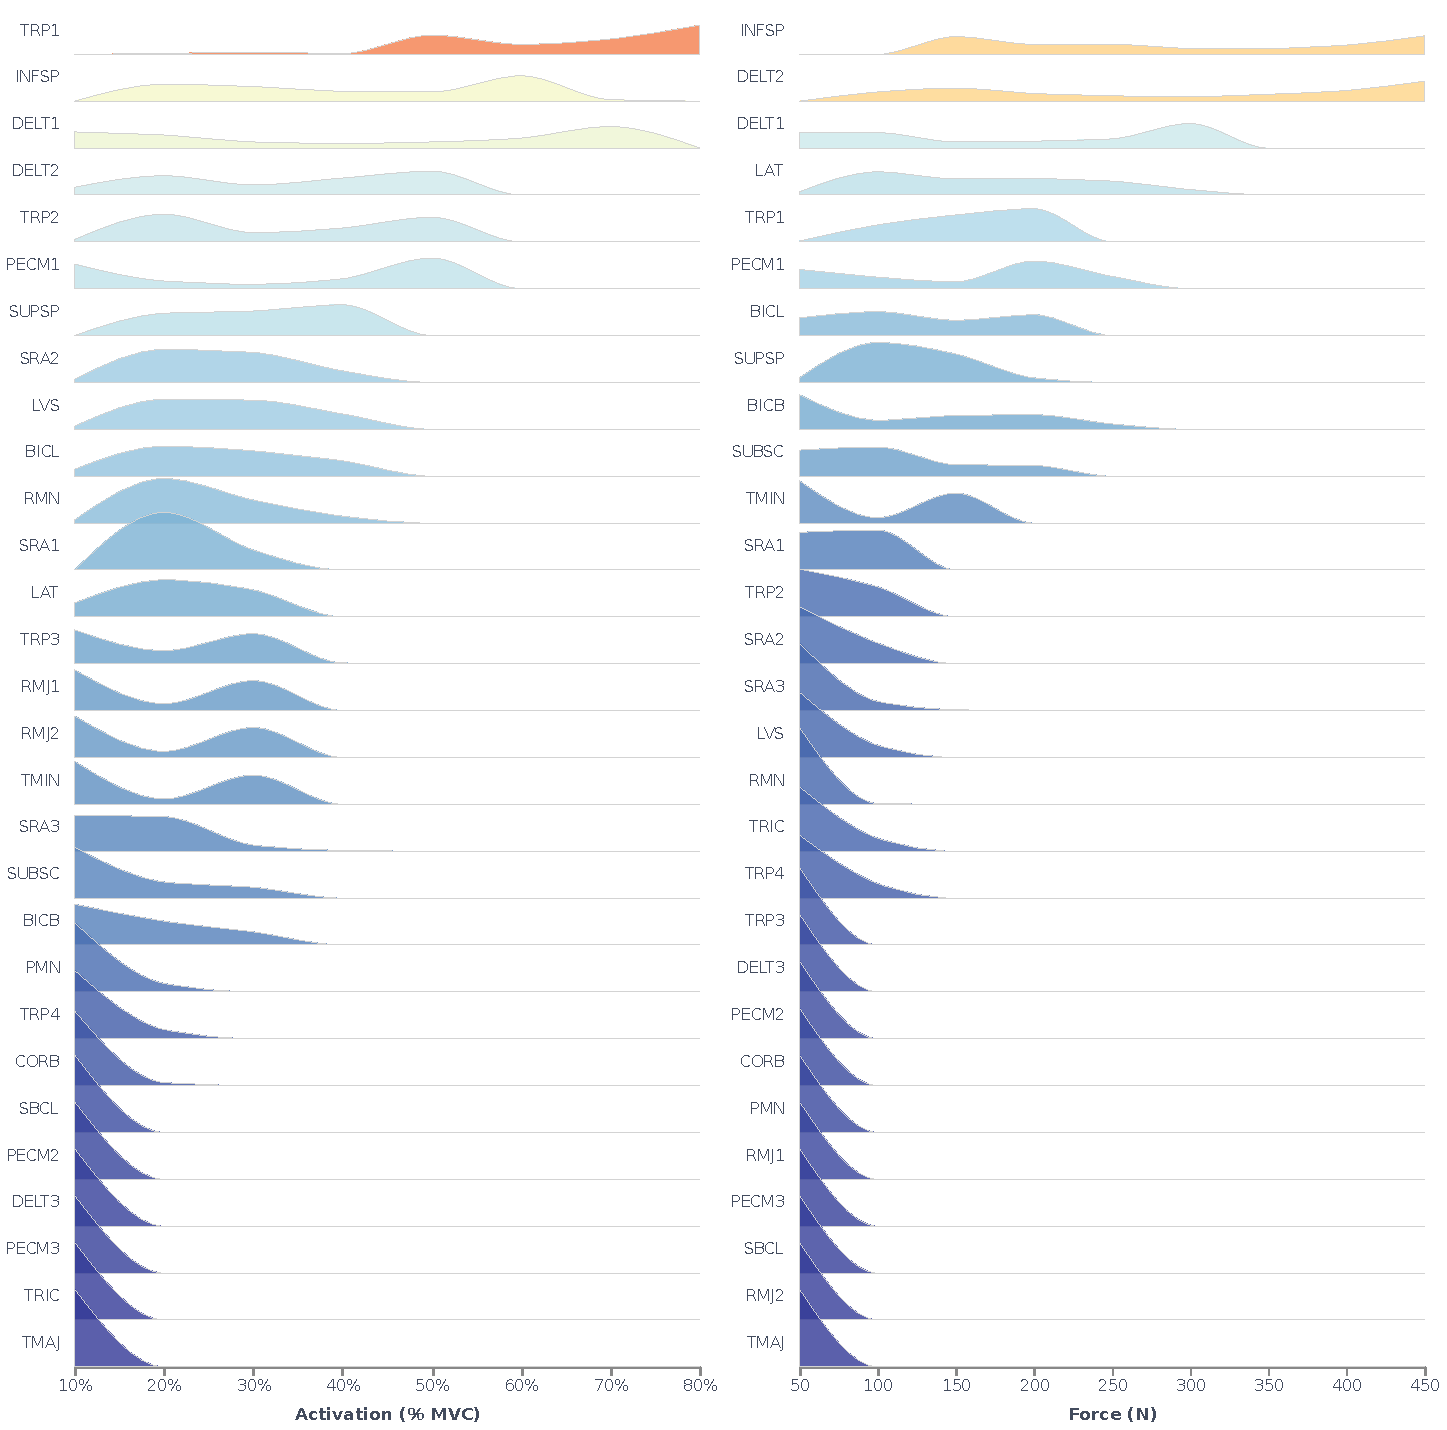
\includegraphics[width=1\linewidth]{fig/dist.pdf}
    \caption{Distribution of muscle activations (left panel) and muscle forces (right panel) for each muscle of the musculoskeletal model.
    The muscles are classified in descending order.
    The distribution is approximated by kernel density estimation and normalized so that the sum of each distribution is equal to 1.
    muscle abbreviations are defined in~\ref{subsec:muscle-abbreviations}}
    \label{fig:dist}
\end{figure}

\subsection{Sex and mass main effects}\label{subsec:sex-and-mass-main-effects}

The sum of muscle activations (Figure~\ref{fig:sum_effects}, top panel) is higher in women during the dropping phase (sex main effect from 55 to 99\%; $+202$\%~MVC; $p<0.001$; $\textrm{ES} = 0.61$ [medium]) and with a 12~kg box during the pulling phase (mass main effect from 8 to 23\%; $+146$\%~MVC; $p<0.001$; $\textrm{ES} = 0.73$ [medium]).
Similarly, the sum of muscle forces (Figure~\ref{fig:sum_effects}, bottom panel) is higher in women during the dropping phase (sex main effect from 77 to 99\%; $+763$~N; $p<0.001$; $\textrm{ES} = 0.59$ [medium]) and with a 12~kg box during the pulling phase (mass main effect from 8 to 24\%; $+535$~N; $p<0.001$; $\textrm{ES} = 0.74$ [medium]).
The 12~kg box also generates higher muscle forces during the dropping phase (mass main effect from 68 to 79\%; $+614$~N; $p = 0.002$; $\textrm{ES} = 0.49$ [small]).

\begin{figure}[H]
    \centering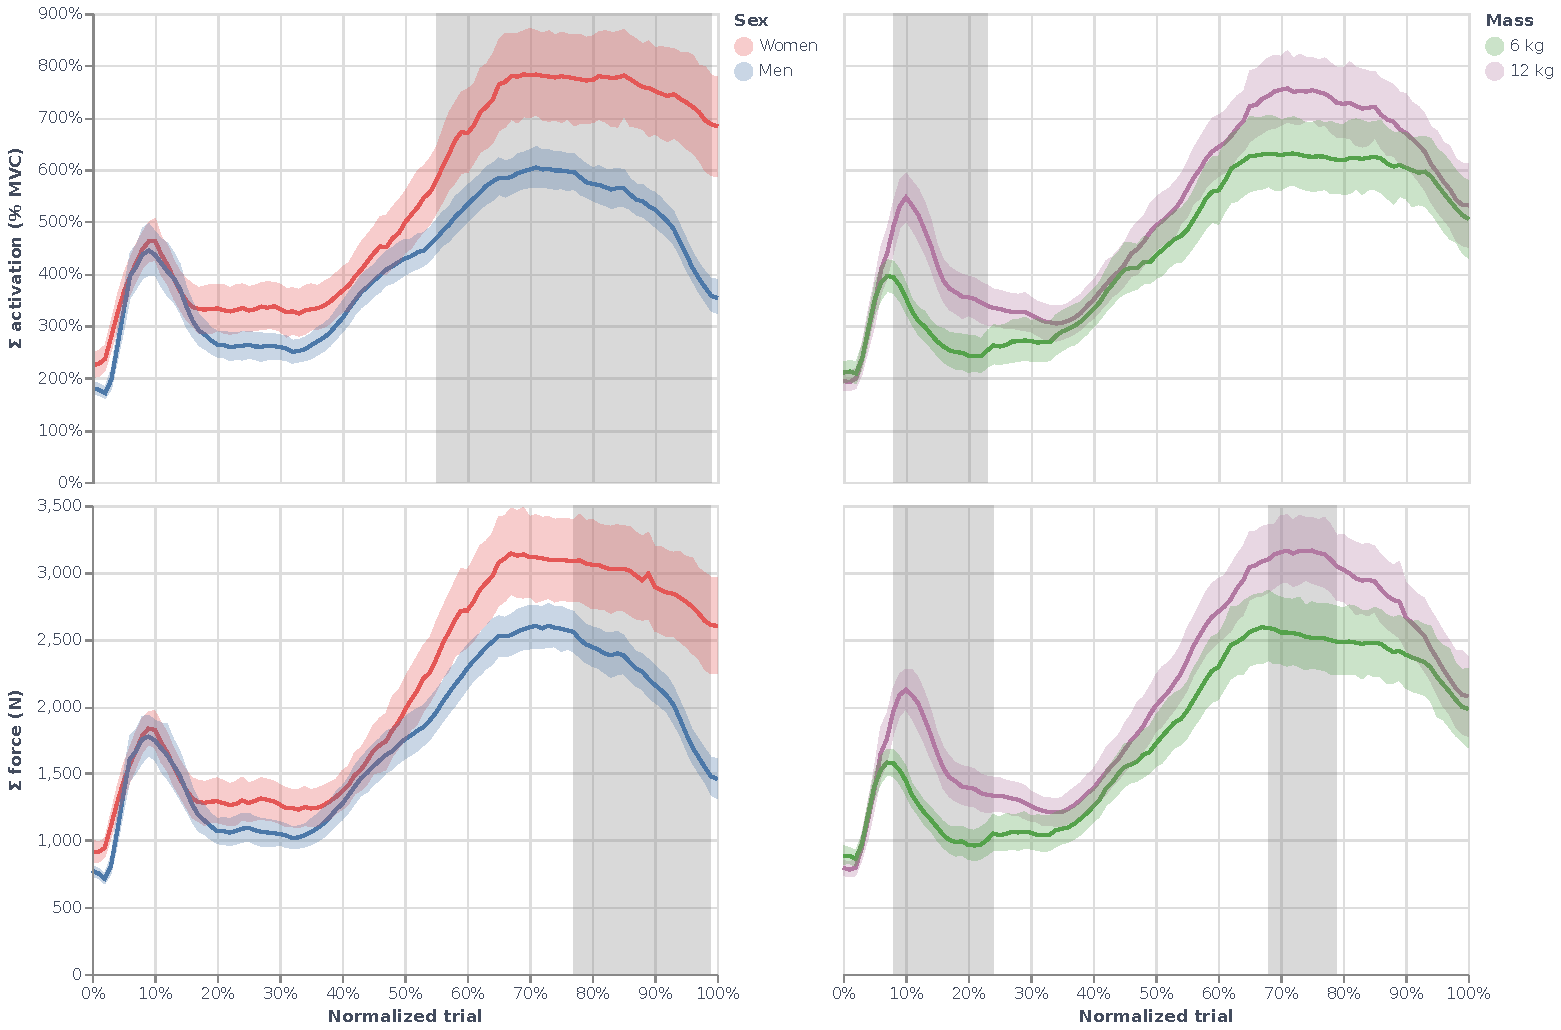
\includegraphics[width=1\linewidth]{fig/sum_effects.pdf}
    \caption{Mean (lines) and 95\% confidence interval (areas) of the sum of muscle activations (upper panels) and sum of muscle forces (lower panels) with the sex (left panel: women in red and men in blue) and mass (right panel: 6~kg in green and 12~kg in purple) main effects.
    A grey area is represented in the presence of a significant effect over time.}
    \label{fig:sum_effects}
\end{figure}

The density of high intensity muscle activations (Figure~\ref{fig:ecdf_effects}, upper panel) is higher in women (sex main effect from 65 to 95\textsuperscript{th} percentiles; $+13$\%~MVC; $p<0.001$; $\textrm{ES} = 0.51$ [medium]) and with a 12~kg box (mass main effect from 90 to 99\textsuperscript{th} percentiles; $+13$\%~MVC; $p<0.001$; $\textrm{ES} = 0.56$ [medium]).
The density of high muscle forces (Figure~\ref{fig:ecdf_effects}, bottom panel) is also higher in women (sex main effect from 58 to 80\textsuperscript{th} percentiles; $+10$~N; $p = 0.001$; $\textrm{ES} = 0.39$ [small] and from 88 to 99\textsuperscript{th} percentiles; $+68$~N; $p = 0.002$; $\textrm{ES} = 0.44$ [small]) and with a 12~kg box (mass main effect from 67 to 97\textsuperscript{th} percentiles; $+27$~N; $p < 0.001$; $\textrm{ES} = 0.24$ [small]).

\begin{figure}[H]
    \centering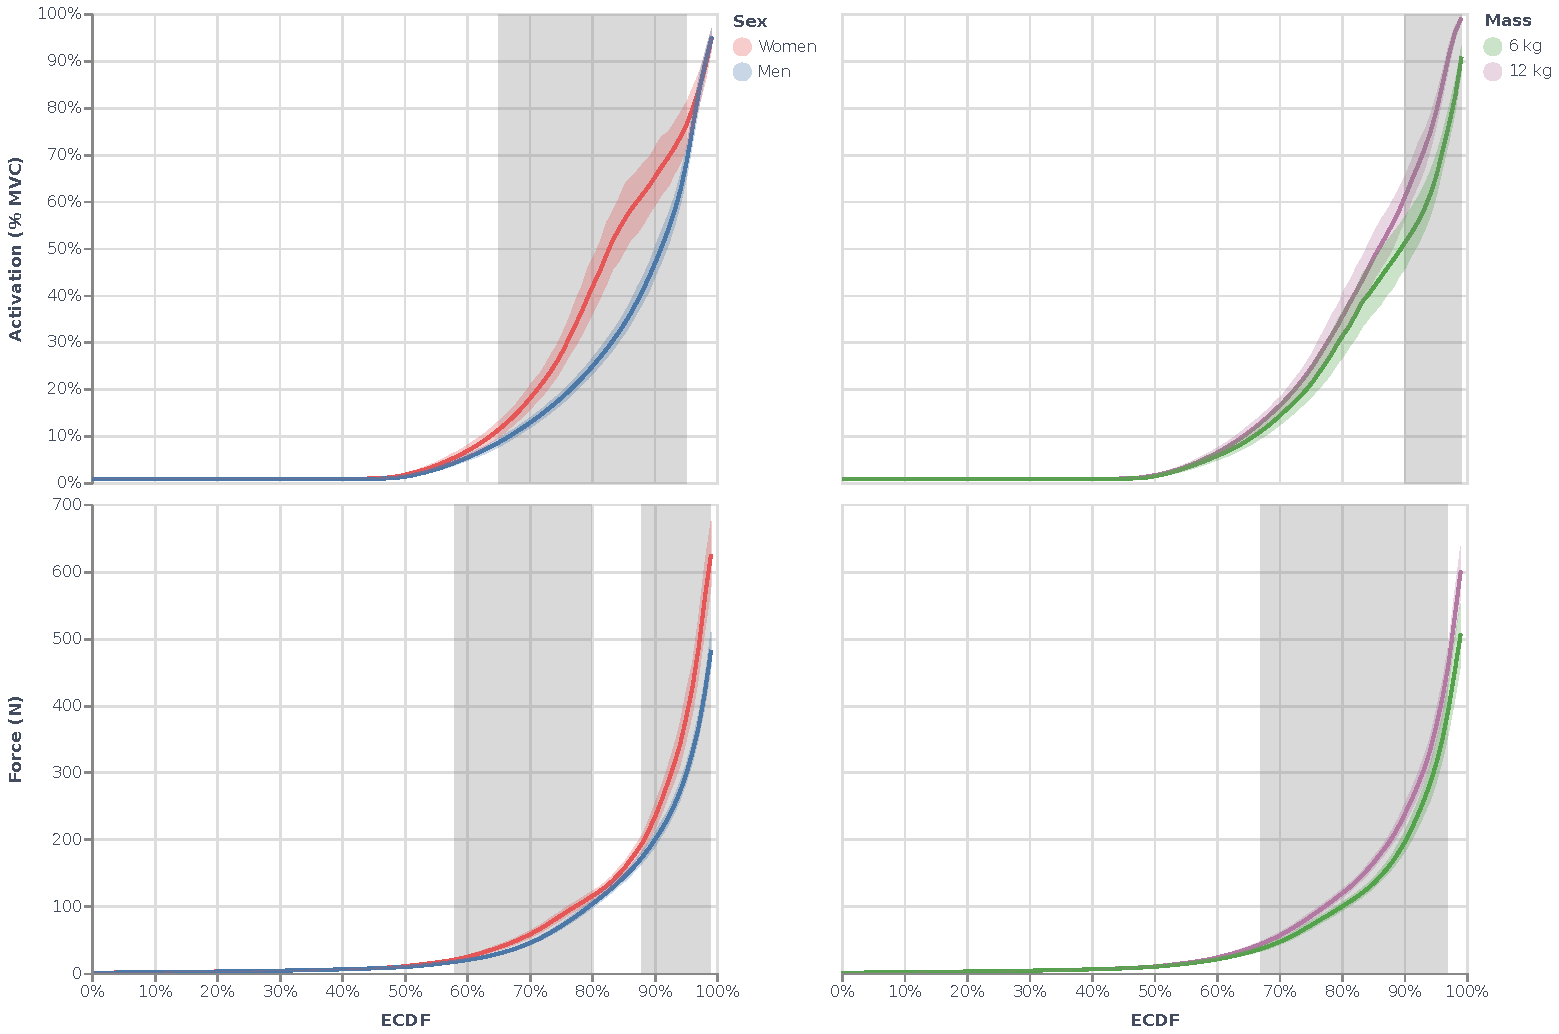
\includegraphics[width=1\linewidth]{fig/ecdf_effects.pdf}
    \caption{Mean (lines) and 95\% confidence interval (areas) of the empirical cumulative distribution function (\textsc{ecdf}) of muscle activations (upper panels) and muscle forces (lower panels) with the sex (left panels: women in red and men in blue) and mass (right panels: 6~kg in green and 12~kg in purple) main effects.
    The \textsc{ecdf} evaluated at $x$ is defined as the fraction of the data points that are $\leq x$.
    A grey area is represented in the presence of a significant effect.}
    \label{fig:ecdf_effects}
\end{figure}

The relative time spent beyond a shear-compression dislocation ratio (Figure~\ref{fig:dislocation}) is higher in women (sex main effect; $+5$\%; $p = 0.045$; $\textrm{ES} = 0.29$ [small]) and remains constant between 6 and 12~kg (no mass main effect).

\begin{figure}[H]
    \centering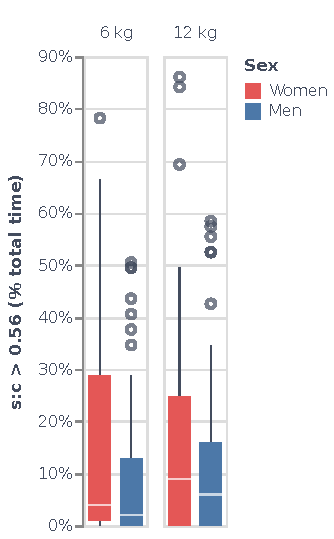
\includegraphics[width=0.3\linewidth]{fig/dislocation.pdf}
    \caption{Boxplot of the relative time spent beyond a shear-compression dislocation ratio by sex (women in red and men in blue) and mass (6~kg on the left panel and 12~kg on the right panel) with median (horizontal lines), first-third interquartile range (bars), first-third interquartile range multiplied by 1.5 times the interquartile difference [$\textrm{Q1} - 1.5 \times \textrm{IQR}; \textrm{Q2} + 1.5 \times \textrm{IQR}$] (vertical lines).
    Data beyond the end of the whiskers are considered outliers (points).}
    \label{fig:dislocation}
\end{figure}